\documentclass[11pt, a4paper, twoside]{Thesis}

\usepackage{subcaption}
\usepackage{amsmath}
\usepackage{tocbibind}
\usepackage{multirow}
\usepackage{setspace}
\usepackage{todonotes}
\usepackage{packages/algorithm2e}
\usepackage{textcomp}
\usepackage{xcolor}


\setlength{\parindent}{0.7cm}

\makeatletter
\DeclareRobustCommand\onedot{\futurelet\@let@token\@onedot}
\def\@onedot{\ifx\@let@token.\else.\null\fi\xspace}

\def\eg{\emph{e.g}\onedot} \def\Eg{\emph{E.g}\onedot}
\def\ie{\emph{i.e}\onedot} \def\Ie{\emph{I.e}\onedot}
\def\cf{\emph{c.f}\onedot} \def\Cf{\emph{C.f}\onedot}
\def\etc{\emph{etc}\onedot} \def\vs{\emph{vs}\onedot}
\def\wrt{w.r.t\onedot} \def\dof{d.o.f\onedot}
\def\etal{\emph{et al}\onedot}
\makeatother

\newcommand{\argmax}{\operatornamewithlimits{argmax}}
\newcommand{\argmin}{\operatornamewithlimits{argmin}}
\newcommand{\abs}[1]{\left\lvert#1\right\rvert}
\newcommand{\norm}[1]{\left\lVert#1\right\rVert}
\newcommand{\listofalgorithmes}{\tocfile{\listalgorithmcfname}{loa}}

\begin{document}
% *************** Front matter ***************
\frontmatter

\title  {Rendering and Streaming of
Bidirectional Texture Functions }

\authors  {\texorpdfstring
            {{Oleksandr Sotnychenko}}
            {Oleksandr Sotnychenko}
            }
\addresses  {\groupname\\\deptname\\\univname}  % Do not change this here, instead these must be set in the "Thesis.cls" file, please look through it instead
%\usdate
\date       {Saarbr\"ucken, \today }
\subject    {}
\keywords   {}

\maketitle

%\newpage
%\mbox{}
%\thispagestyle{empty}
%\newpage

\setstretch{1.3}

\thispagestyle{empty}

\section*{Eidesstattliche Erkl\"{a}rung}
Ich erkl\"{a}re hiermit an Eides Statt, dass ich die vorliegende Arbeit selbstst\"{a}ndig verfasst und keine
anderen als die angegebenen Quellen und Hilfsmittel verwendet habe.

\vspace{0.60cm}
\section*{Statement in Lieu of an Oath}
I hereby confirm that I have written this thesis on my own and that I have not used any other media or
materials than the ones referred to in this thesis.
\vspace{1.5cm}

\section*{Sperrvermerk}


\vspace{0.60cm}
\section*{Blocking Notice}

\vspace{3cm}

\begin{flushright}
\noindent Saarbr\"{u}cken, \today
\hfill
Oleksandr Sotnychenko
\end{flushright}

\clearpage  % Declaration ended, now start a new page
%% ----------------------------------------------------------------

\newpage
\mbox{}
\thispagestyle{empty}
\newpage

% The Abstract Page
\addtotoc{Abstract}  % Add the "Abstract" page entry to the Contents
\abstract{
\addtocontents{toc}{\vspace{1em}}  % Add a gap in the Contents, for aesthetics

Bidirectional Texture Function (BTF) is a 6-dimensional function that depends on spatial position on a texture surface and on light and camera views.
An appearance of realistic materials drastically changes with light and camera variations.
 BTF can model reliable presentation of such materials and capture reflectance properties with a wide range of illumination variations.

In this work we present WebGL-based rendering of BTF in a web-browser. 
An ever-growing number of mobile devices that use web-browser implies that rendering must be possible for hardware with very limited capabilities.
Also, due to enormous size of BTF - compression step is inevitable. 
We employ a principal component analysis to compress the data, which allows for rendering of BTF with interactive frame rates. 
To provide immediate feedback to the user we provide a solution to stream the BTF data and to progressively enhance the rendering quality while the data downloads. 






}
\clearpage
%% ----------------------------------------------------------------
\newpage
\mbox{}
\thispagestyle{empty}
\newpage

\setstretch{1.3}  % Reset the line-spacing to 1.3 for body text (if it has changed)

% The Acknowledgements page, for thanking everyone
\acknowledgements{
\addtocontents{toc}{}  % Add a gap in the Contents, for aesthetics    \vspace{1em}


I am deeply grateful to my adviser Jan Sutter for giving me motivation, for sharing his experience with me and for his continuous support in writing my thesis.
I am thankful to my supervisor Prof. Dr. Philipp Slusallek for inspiring me to write the thesis in the field of Computer Graphics and providing me with valuable pieces of advice.
Special thanks go to Kristian Sons and Felix Klein for giving me a continues support and for providing me with directions.

I would like to express my sincere gratitude to Saarland University for providing excellent studying possibilities. 
I am thankful to the German Research Center for Artificial Intelligence for very pleasant working atmosphere.

 Last but not least, I am especially thankful for my parents and friends, who supported me during my studies.






}
\clearpage  % End of the Acknowledgements
%% ----------------------------------------------------------------
\newpage
\mbox{}
\thispagestyle{empty}
\newpage

\thispagestyle{empty}
\emph{To my family.}
\clearpage

\newpage
\mbox{}
\thispagestyle{empty}
\newpage

\setstretch{1}
\begin{spacing}{0.1}
\pagestyle{fancy}
\tableofcontents
\newpage
\listoffigures
\newpage
%\listoftables
%\newpage
%\listofalgorithmes
\end{spacing}

\clearpage

\setstretch{1.3}
% *************** Main matter ***************
\mainmatter

\chapter{Introduction}
\label{chapter:introduction}

One of the main goals in computer graphics is realistic rendering. 
Even though computer graphics is constantly improving, we are still quite away from reality because material representation in a traditional way lack important realistic properties. 
A 2-D texture in conjunction with a shading model is a conventional way to represent material appearances in rendering.
Real-world materials surfaces on the other hand consist of surface meso-structures, i.e. intermediate in between micro and macro structures.
Meso-structures are responsible for fine-scale shadows, self-occlusions, inter-reflection, subsurface scattering and specularities.
Also, reflectance and the look of real-world materials can drastically change when camera and light directions vary.

One of the possible solution to represent such material attributes is to use sophisticated light functions, for instance a Bidirectional Texture Function (BTF). 
 A BTF is a 6-dimensional function that depends on camera and light directions as well as on spatial texture coordinates. 
The BTF conceptually extends traditional 2-D textures by the dependence on light and camera directions.
This function is usually acquired as a data-set of thousands of images that cover discrete light and camera directions.
Due to the enormous size of that data direct renderings even on modern hardware without any compression is impractical.
Fortunately, many techniques exist to deal with the huge size of BTFs, i.e. compression methods.


In this thesis, we use \emph{WebGL} for real-time rendering of BTF in the Web.
Even though 3-D graphics for the Web becoming more and more popular. BTFs are rarely used realistic rendering, due to their huge size and the overall computational effort needed for rendering,
including decompression of the data and interpolation of camera and light directions.
Such demanding computational effort is time consuming, especially for on mobile-devices.

And the problem which arises when rendering BTFs in a Browser is the transmission of the data.
Before rendering on the client side, the transmission of the data has to be finished.
Even the transfer of a compressed BTF data can take a considerable amount of time. 
The compressed BTF can be tens of megabytes in size.
Because users are eager to see a result, especially on the Web, we use a streaming solution to deliver the data as quickly as possibly, while steadily increasing the resulting image.
 \emph{Web-Sockets} are the state of the art technique for streaming and are supported by most of today's browsers.
With \emph{Web-Sockets}  a  full-duplex communication is available for the server and the client, which is faster than traditional HTTP-based methods. 
This promises fast and reliable solution for real-time performance in \emph{WebGL}-based application.

In this thesis we use a PCA for compression, which allows for a considerably good compression ratio with low decompression error.
Also, it is well suited for real-time rendering and streaming.

We implemented WebGL demo web-application and \emph{Web-Sockets} server for streaming purposes.



\section{Related Work}
\label{section:related_work}

Nowadays, Web technologies are able to support WebGL \cite{webgl}, which is a JavaScript API for rendering 3D content.
WebGL provides  vertex and fragment shaders  for creating highly realistic rendering results.
New standards for 3D graphics in context of HTML domain are evolving, for instance such as XML3D \cite{xml3d}.
XML3D allows for embedding 3D graphics into HTML pages. XML3D is based both on XML and WebGL.
It allows for declaring 3D scenes elements in the context of HTML pages.
Web programmers can apply their existing knowledge (i.e. about DOM, XML, CSS) to include 3D graphics in the HTML content by using XML3D.
Currently XML3D  natively supported by  Firefox and Google Chrome browsers on Linux and Windows.
 
Most of previous work that used BTFs for realistic rendering were primarily intended  for offline applications.
However, their approach is not suitable in the context of the Web, due to the data transfer between the server and a client.
  Schwartz \emph{et. al.} \cite{webglbtfstreaming} presented a work in which compressed BTF data is streamed from the server to a client.
 The streaming over the Internet is done by means of HTTP streaming, i.e. the web-application requests the data in small chunks.
 With each new chunk of the BTF data the rendering quality of the 3D object is progressively enhanced.
 We on the other hand, use \emph{Web-Sockets} to improve application performance compared to HTPP streaming, by reducing the network latency and streaming the data in a binary form.

 
Existing BTF compression methods are reviewed by Haindl \emph{et. al.} \cite{haindl, haindl_visual}.
A trade-off has to be made between the rendering quality and compression rate depending on the intended application.
 Our compression method is related to the PCA RF (Principal Component Analysis Reflectance Field) method, which was introduced by Sattler \emph{et. al.} \cite{star2004}.
This method allows for real-time performance with realistic rendering quality. 
Sattler performs PCA on each of the $n$ camera directions separately. We on the other hand, perform PCA on $k$ neighbour camera directions at once.
In Haindl's review \cite{haindl} PCA based methods achieve better or at least equal reconstruction results than most other methods.
Compression rates of PCA methods are not as high as those of other methods. However, those methods, which produce better compression rates, have worse quality than PCA based methods.



\section{Outline}
\label{section:outline}

\begin{figure}[h]
 \centering
 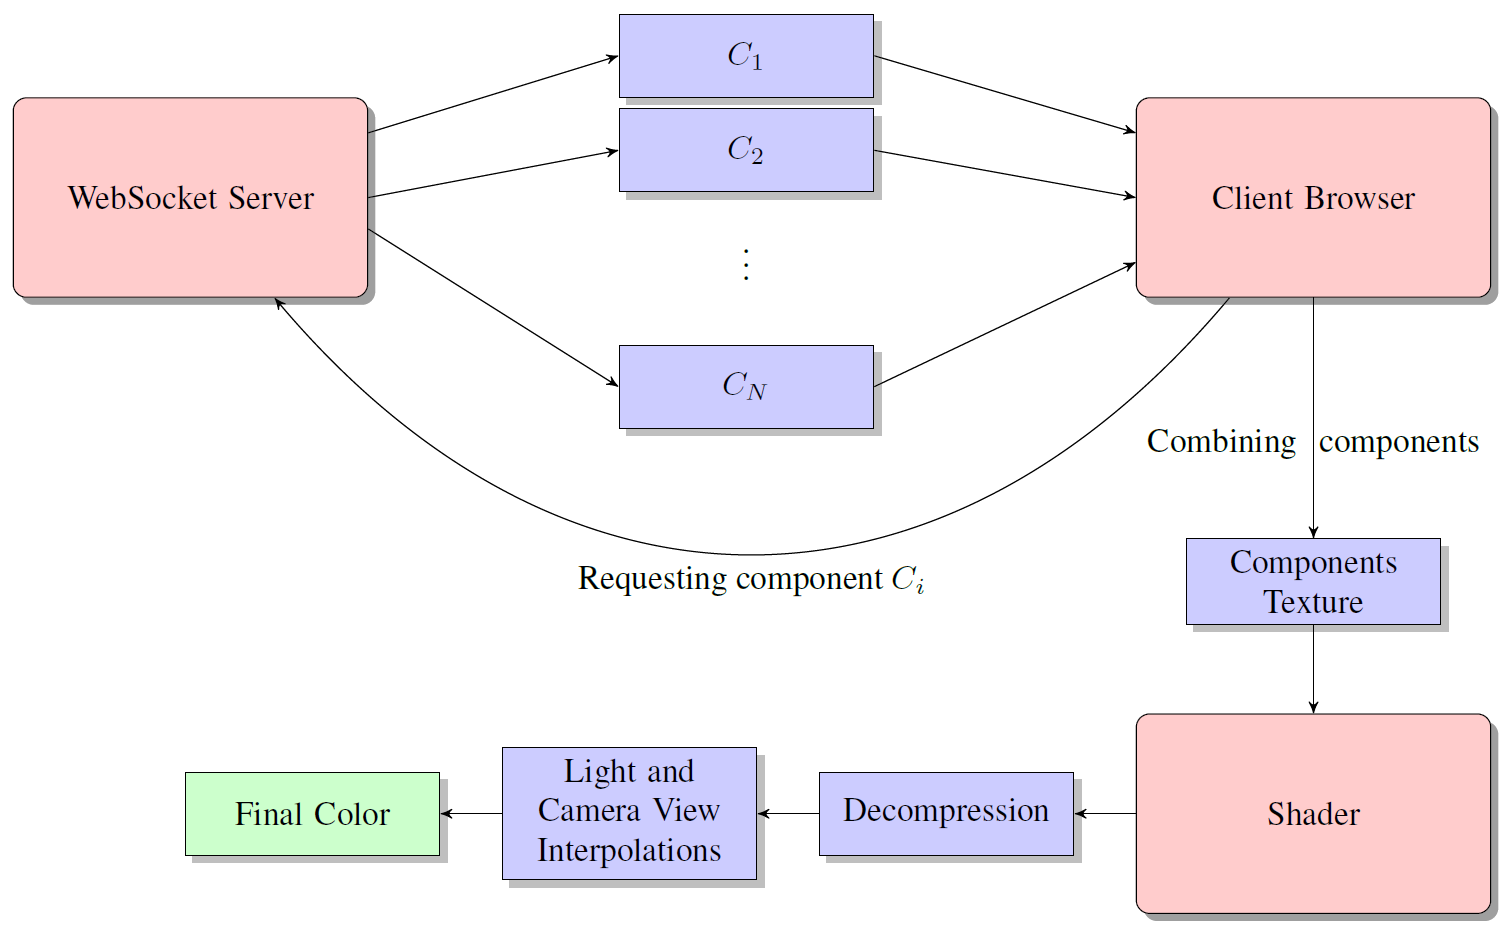
\includegraphics[width=1.0\textwidth]{figures/overview}
 \caption[Model Overview ] {
 	{\bf Model Overview}

	
	}
 \label{fig:overview}
\end{figure}




\clearpage


\chapter{A hierarchy of scattering functions}
\label{chapter:appearance}

In this chapter we will review a hierarchy of scattering functions. 
Scattering functions describe for a surface how incoming and outgoing directions of the light are related \cite{dong}.
Such functions are possible to measure for a given object.
After obtaining the data, scattering functions can provide all the necessary information to render the material appearance. 
Due to diversity of material properties, different functions were introduced.  
In order to chose suitable scattering function for capturing certain scattering effects for a particular type of material,
it is important to be aware of the hierarchy of scattering functions.

	
\section{Light material interaction}
\label{section:light}	
Before defining any scattering functions of light the basics light-material interaction.
Generally speaking, when light hits a material's surface, a sophisticated light-matter process happens.
Such process depends on physical properties of the material as well as on physical properties of light\cite{wynn}. 
For instance, an opaque surface such as wool will reflect light differently than a smooth surface with high specularities such as metal. 

 When light makes a contact with a material, three types of interactions may occur: light \emph{reflection}, light \emph{absorption} and light \emph{transmittance}. 
 Light \emph{reflection} is the change in direction of light at an interface between two different media so that light returns into the medium from which it originated.
 Light \emph{absorption} is a process when a light is being taken up by a material and transformed into internal energy of the material, for instance thermal energy.
 When a material is transparent, light \emph{transmittance} can occur.
 It means, that the light travels through the material and exits on the opposite side of the object. 
  Figure 2 demonstrates these 3 types of interactions.
  
 Because light is a form of energy, conservation of energy says that \cite{wynn}
 \begin{center} 
\emph{incident light at a surface = light reflected + light absorbed + light transmitted}
 \end{center}
 


\section{General Scattering Function}
\label{section:grf}
 
To define the general scattering function(GSF) imagine the light-wave hitting the surface at time $t_{i}$ and position $x_{i}$ and with wavelength $\lambda_{i}$\cite{star2004}.
 With a given local coordinate system at a surface point, the incoming direction of light can be defined as $(\theta_{i} ,\phi_{i})$.
 Light travels inside the material and exits the surface at position $x_{o}$ and time $t_{o}$, with possibly changed wavelength $\lambda_{o}$ in the outgoing direction $(\theta_{o} ,\phi_{o})$.
  
According to the description we get a GSF
 \begin{center} 
$GSF(t_{i},t_{o},x_{i},x_{0,}\theta_{i} ,\phi_{i},\theta_{o},\phi_{o},\lambda_{i},\lambda_{o})$
 \end{center}
in which  spatial positions $x_{i,o}$ are 2-D variables.
This function describes light interaction for each surface point for any incoming light and outgoing direction at certain time.
The function has 12 parameters! Note that we neglected light transmittance, which would even further complicate the function.


\section{Bidirectional Scattering-Surface Reflectance Distribution Function}
\label{section:BSSRDF}
 Since the measurement, modeling and rendering of a 12-D GSF function is currently not practical, additional assumptions have to be made to simplify the function.
 Usually such assumption are made \cite{star2004}:

\begin{itemize}
 \item light interaction takes zero time ($t_{i}$  = $t_{o}$)
 \item wavelength is separated into the three color bands red, green and blue ($\lambda_{r,g,b}$)
 \item interaction does not change wavelength ($\lambda_{i}= \lambda_{0}$)
\end{itemize}

After mentioned assumptions we get a 8-D bidirectional scattering-surface reflectance distribution function (BSSRDF)
 \begin{center}
$BSSRDF(x_{i},x_{o}\theta_{i} ,\phi_{i}\theta_{o} ,\phi_{o})$
 \end{center}


BSSRDF describes various light interactions for heterogeneous both translucent and opaque materials.
That is why BSSRDF can be used for rendering materials such as skin, marble, milk and other objects which do not look realistic without subsurface scattering. 
Subsurface scattering is a process when light penetrates an object at an incident point, travels inside the object and exists at a different point of the object.

\section{Bidirectional Texture Function}
\label{section:btf}
If we simplify further and assume that

\begin{itemize}
 \item light entering a material exits at the same point $x_{i}=x_{o}$, while internal subsurface scattering is still present
\end{itemize}

we will get a 6-D bidirectional texture function (BTF).

Subsurface scattering, self-occlusion, self-shadowing  are still present, now it just comes pre-integrated, i.e. it can be defined through BSSRDF \cite{star2004}:
 \begin{center}
$ BTF(x,\theta_{i} ,\phi_{i},\theta_{o} ,\phi_{o})=\int_{S}BSSRDF(x_{i},x,\theta_{i} ,\phi_{i},\theta_{o} ,\phi_{o}) dx_{i}$
 \end{center}
  The assumption that $x_{i}=x_{o}$ simplifies measuring, modeling and rendering of the scattering function. 
 As we can see the BTF integrates subsurface scattering from neighbouring surface locations. 

\section{Bidirectional Subsurface Scattering Distribution Function}
\label{section:BSSDF}

Another possible reduction of the 8-D BSSRDF is to assume that we deal with a homogeneous surface \cite{dong}, i.e.
\begin{itemize}
 \item subsurface scattering depends only on relative surface positions of incoming and outgoing light $(x_{i}-x_{o})$
\end{itemize}
  Simply saying it means that scattering do not vary over a surface.
 With such assumption we get a 6D function that known as a bidirectional subsurface scattering
distribution function (BSSDF).
 \begin{center}
$BSSDF(x_{i}-x_{o},\theta_{i} ,\phi_{i},\theta_{o} ,\phi_{o})$
 \end{center}
 BSSDF represents homogeneous materials for which subsurface scattering is a significant feature of their overall appearance.
 For instance, BSSDF accounts for objects such as water, milk, human skin, and marble.

\section{Bidirectional Reflectance Distribution Function}
\label{section:brdf}

If we assume the following for a BSSDF that

\begin{itemize}
 \item there is no spatial variation 
 \item no self-shadowing
 \item no self-occlusion
 \item no inter-reflections
 \item no subsurface scattering
 \item energy conservation
 \item reciprocity  $BRDF(\theta_{i} ,\phi_{i},\theta_{o} ,\phi_{o})$=$BRDF(\theta_{o} ,\phi_{o},\theta_{i} ,\phi_{i})$.
\end{itemize}

 we get a 4-D bidirectional reflectance distribution function (BRDF)
 \begin{center}
$BRDF(\theta_{i} ,\phi_{i},\theta_{o} ,\phi_{o})$.
 \end{center}
Nicodemus et al. \cite{Nicodemus} was the one who proposed the BRDF. 
Two principal properties of the BRDF were introduced, i.e. \emph{energy conservation} and \emph{reciprocity}. 
\emph{Energy conservation} law states that the total amount of outgoing light from a surface cannot exceed the
original amount of light that arrives at the surface \cite{wynn}. 
 \emph{Reciprocity} says that if we swap incoming and outgoing directions BRDF stays the same.
If either of these conditions are not satisfied then such BRDF is called \emph{apparent} BRDF (ABRDF) \cite{abrdf}.

It is quite difficult to create a mathematical model for a BRDF that satisfies reciprocity,
energy conservation and the same time produces realistic images. However, most BRDF's models do not satisfy these conditions and still get plausible rendering results.
For instance, Phong model is the most well-known shading model in computer graphics. 
The traditional Phong model satisfy neither energy conservation nor reciprocity, but can still render many materials realistically plausible.
Usually, such materials are of opaque and flat nature, for example plastic materials.
The Phong model is an empirical model and is designed to fit the original function, often based on simple formulas which were derived from observations.


\section{Spatially Varying Bidirectional Reflectance Distribution Function}
\label{section:svbrdf}
If spatial dependence for BRDF takes place, we get a 6-D spatially varying BRDF (SVBRDF)


 \begin{center}
$SVBRDF(x,\theta_{i} ,\phi_{i},\theta_{o} ,\phi_{o})$.
 \end{center}
 Assumptions are the same as for the BRDF, except now spatial dependence is present.
 
A SVBRDF is closely related to a BTF. The SVBRDF and the BTF almost the same scattering function, the difference is in scattering process. 
Changes in scattering at local position $x$ for the BTF are influenced from neighbouring 3D surface geometry, as a result the self-shadowing, masking and inter-reflections are captured by the BTF.
On the other side, the spatial dependence of a SVBRDF describes variations in the optical properties of a surface \cite{haindl_visual}.


 
A SVBRDF represents structures at micro-scale level, which corresponds to near flat opaque materials. On the other side, a BTF capture structure both at macro and micro scales.
 That means that the BTF takes into account influences from local neighbourhood structures. Even though measurement, compression, rendering are more efficient for the SVBRDF, 
 the BTF can produce better visual results. \cite{haindl_visual}

\section{Summary of scattering functions}
\label{section:attrib}
In practice, an advantage of simpler scattering function is a computation efficiency, 
while a disadvantage is a reduction of visual quality. 
But, development of the graphics hardware is always improving and 
as a result this encourages to use sophisticated scattering functions, which provide improvement in realistic material rendering. 
 
However, a complex material representation introduces additional constraints on the data measurement as well as modeling becomes more challenging.
For instance, till now a GRF has not been measured and still stays as a state-of-the-art problem.
In practice, the appropriate scattering function depends on the specific application.
For instance, a scene with various textures can be rendered with different scattering functions. 
Simpler materials that do not have complex scattering features can be rendered with a 2-D textures in conjunction with BRDFs model. 
If the material cannot be presented realistic without subsurface scattering, masking, self-reflections then typically such materials require high quality representations (BTF,SVBRDF).
However, these advanced material representations are very complex.
In practice a tradeoff between visual quality, measurement, data size and rendering cost is inevitable. 
Ideally high visual quality is preferred with low rendering computational cost.



\clearpage

\chapter{Bidirectional Texture Functions}
\label{chapter:stateOfArt}


\section{Acquisition}
\label{chapter:acquisition}

BTF acquisition is not a non-trivial task as it requires special acquisition setup. 
There are only a few measurement systems \cite{star2004,schwartz,dana,Kaleidoscope,Koudelka,statistical_acq} exist, but as the interest in realistic material rendering using BTFs is growing, measurement systems are developing.
In this chapter we will review how in general BTF data acquisition is done, which post-processing steps are made, and advantages and disadvantages of existing measurement systems. 
We will also review publicly available BTF datasets.

\subsection{General Acquisition Methods}
\label{section:General_acquisition}	
All the mentioned BTF acquisition systems share the same idea in the data acquisition, i.e. capturing the appearance of a flat square slice of the material surface under varying light and camera directions.
The material surface is usually sampled over a hemisphere above the material slice as shown in Figure \ref{fig:acquisition_example}.
Depending on the material's reflectance properties sampling distribution may vary, e.g. the sampling distribution can be dense in regions where specular peaks in the light reflection occur. 
Then, if needed, a uniform distribution can be calculated in a post-processing step using interpolation \cite{haindl_visual}.

Digital cameras are used as capturing devices. Depending on the setup the number of cameras can vary.
 If there is only one camera \cite{star2004,statistical_acq,dana}, it usually moves on a robotic arm or rail-trail system around the hemisphere above the sample\cite{star2004}. 
 The advantage of this approach is that it is less expensive and can suit low-budget applications.
The disadvantage however is the positioning errors that can arise, which influence the overall measurement error. 
Depending on the application light sources can be fixed or moveable.

There are approaches which do not involve camera and light source movement at all.
Schwartz et al. \cite{schwartz} developed a novel measurement system which uses a dense array of 151 cameras, which are uniformly placed on a hemispherical structure.
Flashes of the cameras are used as light sources. Such setup provide a high angular and spatial resolution.

Also, Ngan et al. \cite{statistical_acq} made a setup which does not involve camera movement by placing the planar slices of the material in a form of the pyramid.
Thus, such setup captures the material appearance for 13 different camera views at once. Light directions are sampled by manually-moved electronic flash.
The disadvantage of such setup is that it provides sparse angular resolution, but depending on the application such approach can be plausible.
For example, a material which does not posses high illumination changes can be sparse sampled, thus the reduction of redundant data is achieved.

The material sample is commonly a flat and squared slice, which is placed on the holder plate. To conduct automatic post-processing borderline markers are placed on the holder.
Those markers provide the important information for further post-processing steps such as image rectification and registration.


\begin{figure}[h]
 \centering
 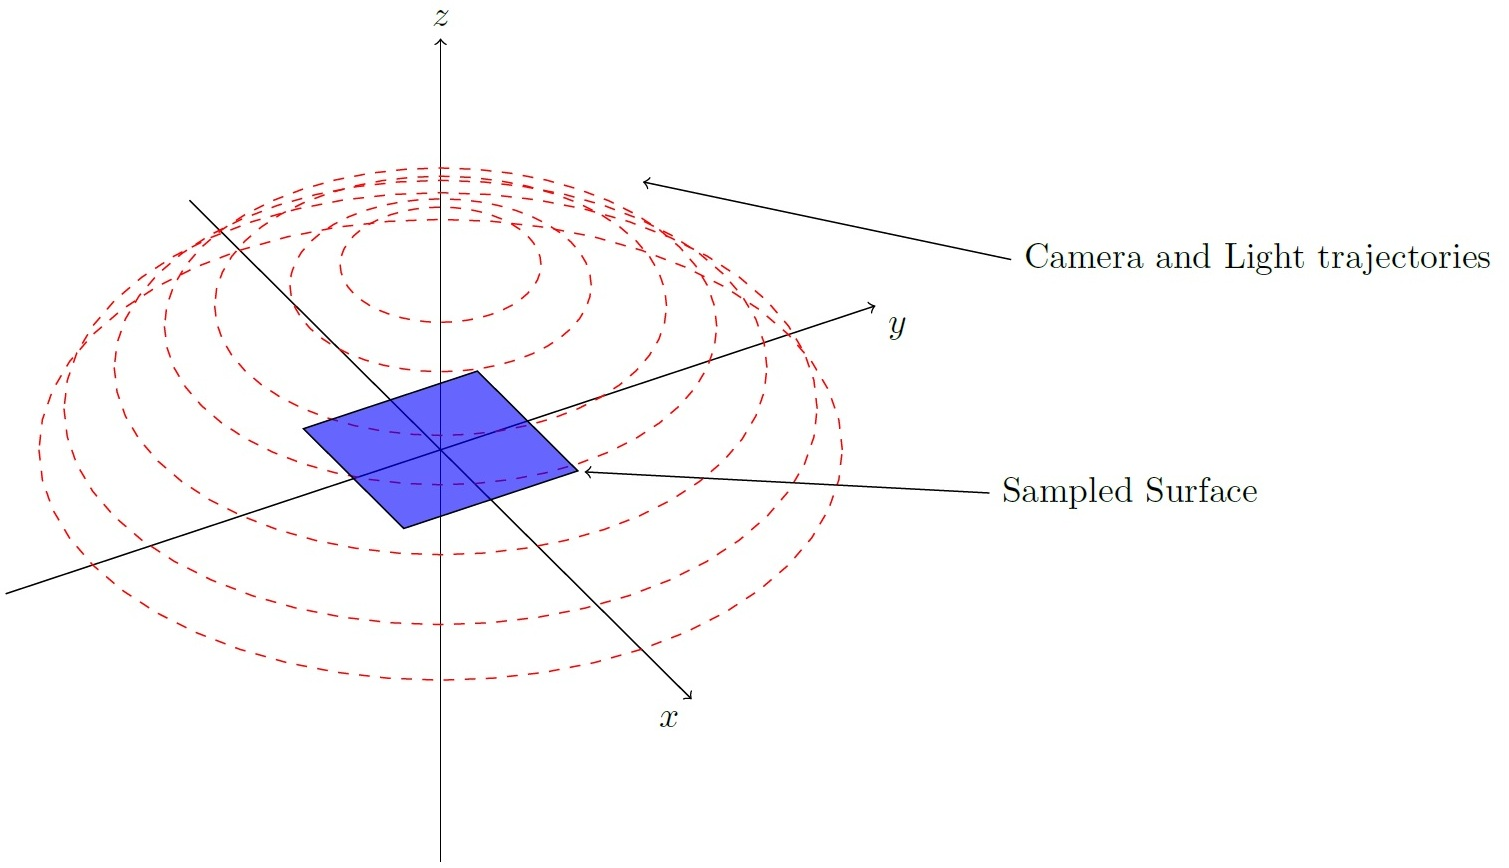
\includegraphics[width=1.0\textwidth]{figures/acquisition}
 \caption[Example of BTF measurement] {
 	{\bf Example of BTF measurement.}

	Camera and light positions share the same trajectories.
	Red dashed circles are the sample positions on the hemisphere. }
 \label{fig:acquisition_example}
\end{figure}

\subsection{Post-processing}
\label{section:Post_processing_acquisition}	
After the measurement is done, the raw data has to be further post-processed, because typically such  data is not ready for compression.
Raw data consists a set of images that are not aligned with each other and are not mutually registered.

When these raw images are obtained under different camera angles $(\theta,\phi)$ they are perspectively distorted \cite{sattler-2003-efficient}.
Thus, all sample images have to be aligned with each other and spatially registered to be further used.
Firstly, borderline markers that were placed around the material sample on the holder plate aid the automatic detection of the material slice.
Then, after the material slices are detected and cropped, they are ready for mutual alignment. This process is called  \emph{rectification}. 
\emph{Rectification} is a process which involves projecting all sample images onto the plane which is defined by the frontal view, e.g. $(\theta _{o} =0,\phi _{o}=0)$.
In other words, all normals of the sample images have to be aligned with their corresponding camera directions, i.e. as if all sample images were taken from frontal view $(\theta =0,\phi=0)$.
The last step is image \emph{registration}, a process of getting pixel-to-pixel correspondence between the images.
Finally all images have to be scaled to an equal resolution.


Even after the proper rectification and registering of the measured data, registration errors can still be present between individual camera directions \cite{haindl_visual}. 
 This happens due to structural occlusion of the material surface. Because of such self-occlusion some geometries structures are not captured by certain camera directions.
 That is why even after rectification images captured from completely different directions are not correctly align. 
Also, registration errors can be caused by both inaccurate camera and material sample positions happened during the measurement processes.


If needed, further processing steps can be done, for instance \emph{linear edger blending} to reduce tiling artifacts \cite{sattler-2003-efficient}.
Also, typical image processing steps may be employed, e.g. noise reduction filters. 


\subsection{Publicly Available BTF Datasets}
\label{section:Publicly_datasets}	

\begin{figure}[h]
 \centering
 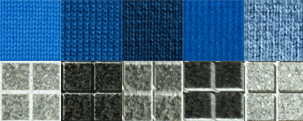
\includegraphics[width=1.0\textwidth]{figures/exampleBTF}
 \caption[Example of BTF measurement] {
 	{\bf BTF example of Bonn Database \cite{btfBonn}.}

	Example how BTF catches rich appearance of the material due to dependencies on light and camera directions. 
	Upper row is a knitted wool, lower is a graved granite stone.}
 \label{fig:exampleBTF}
\end{figure}


The accurate rendering of the material surface is highly depended on the quality of the acquired data, especially for BTF.
There are several properties that are vital for reproducing high quality rendering results.
 BTF datasets can be distinguished by how well image post-processing were done and how good spatial and angular resolutions are.

 
A pioneer in the BTF acquisition was Dana  \emph{et. al.} \cite{curetDataBase}, who measured 61 materials with fixed light and moving camera aided by a robotic arm. 
This procedure resulted in a set of images, which can be seen as a subset of a BTF, which is called surface light field (SLF), see Chapter \ref{section:slf}.
Dana  \emph{et. al.} \emph{CUReT} database is publicly available \cite{curetDataBase}.
For each measured surface Dana  \emph{et. al.} used 205 different combinations of camera and light directions, which resulted in relatively sparse angular resolution.
These datasets are not rectified, but  the authors provide image coordinates to enable rectification. 
 Because of these limitations such BTF dataset are usually used for computer vision purposes, i.e. texture classification  \cite{haindl_visual}.

Based on this BTF measurement system,  Bonn University created their own measuring system \cite{sattler-2003-efficient}.
 The main difference of this system is that the camera moves on a semi-circle rail around the material sample.
Such a setup provides spatially rectificated and mutually registered data, with reasonable angular and spatial resolutions. 
Datasets of the Bonn University \cite{btfBonn} are publicly available and are used in this thesis.


 Consider Figure \ref{fig:exampleBTF}, which illustrates sampled materials from the Bonn database.
The measured surface is being fixed all the time on the sampler holder as shown in Figure \ref{fig:acquisition_example}. 
For each light position, a camera takes a shot of the material while moving from point to point on the hemisphere.
Bonn University datasets have the same trajectory for camera and light positions, i.e. 81 positions on the hemisphere, which resulted in $81\times81=6561$ number of acquired images.
After that the sample images were rectificated and registered, resulting in a set of images with a spatial resolution of $256\times256$.
Typically, the size of one uncompressed BTF is around $1.2$ Gb.



\section{Data Representations}
\label{chapter:representations}




Before doing any further operations on the acquired BTF data it is important to chose a suitable representation for the data.
A suitable presentation can  influence the final quality of BTF rendering and compression ratio enormously.
\subsection{Texture Representation}
\label{chapter:texture_repr}

 The first straightforward representation, as a set of textures can mathematically represented as

{\centering $\,\,\,\,\,\,\,BTF_{Texture}=\left \{I_{(\theta_{i} ,\phi_{i},\theta_{o} ,\phi_{o}) }  \mid  (\theta_{i},\phi_{i},\theta_{o} ,\phi_{o})\in M \right \}$\\}


where $M$ denotes a set of images $I_{(\theta_{i} ,\phi_{i},\theta_{o} ,\phi_{o})}$ measured for different light and camera directions $(i,o)$ accordingly.

Basically, $BTF_{Texture}$ is used for compression methods that do their analysis on the whole sample plane.

\subsection{ABRDF Representation}
\label{chapter:abrdf_repr}

 ABRDF representation is a set of ABRDFs, one ABRDF for each sample position of the material plane. 
 ABRDF was defined in Chapter \ref{section:brdf}. In this case it is called \emph{apparent}, 
 because BTF includes effects such as self-occlusions and sub-surface scattering which violate two basic properties of a BRDF, i.e. \emph{energy conservation} and \emph{reciprocity}.
 
 {\centering $\,\,\,\,\,\,\,\,\,\,\,\,\,\,\,\,BTF_{ABRDF}=\left \{P_{(x) } \,\,\,\,\,\,\,\,\,\,\,\,\,\,\,\,\,\,\mid  (x)\in I_{(\theta_{i} ,\phi_{i},\theta_{o} ,\phi_{o})}\subset \mathbb{N}^{2}\right \}$ \\}
 
 $BTF_{ABRDF}$ denotes a set of $P_{(x)}$ images, i.e. ABRDF for spatial position $x$.


 $BTF_{ABRDF}$ representation allows better pixel-to-pixel comparisons, which can give a big advantage for methods that employ pixel-wise compression, e.g. BRDF based models.

Also, such arrangement provides images with lower variance \cite{haindl}, which can allow better compression results in certain scenarios, e.g. when the material surface is not smooth.

 
\section{BTF Compression Methods}
\label{chapter:compression_methods}



 A measured BTF consists of thousands of images, which require lots of storage space.
In the Bonn  Database \cite{btfBonn} a BTF consists of 8-bit PNG images with a resolution of $256\times256$ sampled for $81\times81$ different camera and light directions.
  Uncompressed BTF occupies approximately $1.2$ GB in size.
 To render a scene with several BTFs and to achieve an acceptable frame-rate becomes practically impossible, especially for low-end hardware.
 Also, as we intent to render BTFs in a web-browser, the data has to be transferred from the server to the client, which means the compact representation of the BTF is utmost importance.
 For our scenario it is important to chose a compression method, that one that allows for real-time decompression, high compression rate while preserving good quality, and separability of compressed BTF data.
 Separability is needed for real-time streaming in a web-browser.  
 As the data is streamed in small chunks and at some point it is important to have an option to render the preview of BTF based on partial data.

There are different methods for BTF compression. Those methods can be categorized as follows:

\begin{itemize}
  \item \emph{Analytic methods} represent BTFs through analytic BRDF models. 
These analytic BRDF models are fitted separately to each texel of the BTF. Such functions  few parameters, thus real-time performance is easily achieved.
However, only these groups of methods can suffer from a decreased rendering quality \cite{haindl}. In addition, it is hard to change parameters in order to control the visual quality. (See Chapter  \ref{section:analytic_methods}).
   \item \emph{Statistical methods}, which belong to methods that reduce dimensionality based on  statistics, for instance based a linear basis decompression method such as PCA (Principal component analysis). 
    PCA based methods are frequently used, because its parameters directly correspond to the trade-off between compression ratio and reconstruction quality.
    Also, PCA is frequently the basis for some more sophisticated methods \cite{webglbtfstreaming}. (See Chapter \ref{section:stat_methods}.)
   \item \emph{Probabilistic models} can extremely compress the original BTF.
   However, the resulted image quality usually suits for flat surfaces. 
   Also, there are problems of implementing these models on the GPU for real-time rendering. (See Chapter \ref{section:prob_methods}.)
 \end{itemize}



 \subsection{Analytic methods}
\label{section:analytic_methods}	
 This group of methods take advantage of the ABRDF representation of a BTF. 
 There is a large number of techniques which allows for a compact representation of BRDFs, which in general can also applied to ABRDFs.
 Each texel of a BTF, i.e. spatial position on the surface are represented as ABRDF. Each of these ABRDFs can be modeled and compressed by any BRDF model.
 
One of the possible ways to model ABRDF is to use \emph{Polynomial Texture  Mapping} (PTM).
Malzbender  \emph{et. al.} \cite{PTM} used this approach which allows for high compression rates and generally good quality. 
However, PTM requires to compute specular and diffuse effects separately. 
The PTM model assumes that the input surface is either diffuse or their specular contribution has been separated beforehand.
For BTFs it can be difficult to separate specular highlights \cite{haindl}.

Haindl  \emph{et. al.} \cite{haindl} applied PTM on Reflectance Fields (RF).
General formula looks the following way (PTM RF):

{\centering$R_{o}(r,i)\approx a_{0}(r)u_{x}^2+a_{1}(r)u_{y}^2+a_{2}(r)u_{x}u_{y}+a_{3}(r)u_{x}+a_{4}(r)u_{y}+a_{5}(r)$\\}

 where $R_{o}$ is the approximated RF for a fixed camera direction $o$ and $u_{x},u_{y}$ are projections of the normalized light vector into the local coordinate system $r=(x,y)$.
 The set of all possible $R_{o}$ is the number of all camera positions, i.e. $n_{o}$. 
 Coefficients $a_{p}$ are fitted by the use of \emph{singular value decomposition} (SVD) for each $R_{o}$ and parameters are stored as a spatial map referred to as a PTM.
 
  This method enables fast rendering and is generally suited for smooth material surfaces.
  However, Malzbender  \emph{et. al.} \cite{PTM} claim that this method produce considerable errors for high grazing angles. 

 
 Another model which produces slightly better visual quality is the polynomial extension of the one-lobe Lafortune model (PLM) \cite{haindl}.


{\centering$Y_{o} (r,i) = \rho_{o,r}(C_{o,r,x}u_{x}+C_{o,r,y}u_{y}+C_{o,r,z}u_{z})_{ }^{n_{o,r}}$\\}

where $w_{i}(\theta_{i}, \phi_{i})=[u_{1},u_{2},u_{3}]^{T}$ is the unit vector pointing from surface to light.
Parameters $\rho,C_{x},C_{y},C_{z},n$ can be computed with a Levenberg-Marquardt non-linear optimisation algorithm \cite{plm}. 
 Filip and Haindl \cite{plm} claim that the one-lobe Lafortune model produces unsatisfactory results for complex ABRDFs.
 Thus, the polynomial extension of the one-lobe Lafortune was introduced (PLM RF):

{\centering$R_{o}(r,i)\approx  \sum_{j=0}^{n} a_{r,o,i,j}Y_{o}(r,i)^j$\\}



PLM RF solves the problem of bad quality for grazing angles and improves the rendering quality compared to PTM RF.
However, statistical based methods produce even better quality compared to above methods but with lower compression rates \cite{haindl}.



  \subsection{Statistical methods}
\label{section:stat_methods}
This group of methods is mostly based on a dimensionality reduction of the data, while preserving the most important information.
The goal of dimensional reduction is to find a new basis which would represent the data with less dimensions and at the same time preserving the important features of the original data.
 The size of the data with the new basis will be decreased.

One of the popular methods used for BTF compression belongs to this group, i.e. \emph{Principal component analysis} (PCA) \cite{Bishop,schneider2004,haindl,webglbtfstreaming,sattler-2003-efficient,mueller-2003-compression,gpu_gems}.
PCA is a linear transformation of the data to a new basis, where each new coordinate (variable) is called a \emph{principal component} \cite{Bishop}.
All new coordinates are mutually orthogonal, i.e. uncorrelated. Components are sorted by decreasing variance, i.e. the first component posses the greatest variance compared to other components. 
 The last components which hold small variations are discarded, because they do not contribute important information.

PCA is a popular approach for compressing BTF. 
Firstly, PCA allows for a strong correspondence between the number of components and the decompression error.
 The correspondence lies in the amount of components used.
 The more components are used for the better decompression error, and vise-verse, a smaller number of components gives better compression ratio, but worse decompression error.
 This allows for an easy  regulation of the trade-off between rendering quality and  compression ratio.
Secondly, a reasonable compression ratio along with a low decompression error can be achieved, e.g. a compression ratio of $1:100$ with an average decompression error of 2\%- 4\% \cite{schneider2004,haindl}.
Thirdly, PCA is suitable for real-time decompression on average GPUs \cite{schneider2004,haindl}. 
It is suitable, because decompression of a single pixel does not depend on other pixels.
 Computation of a single pixel for PCA decompression on the GPU is done by means of linear combinations of estimated PCA parameters, so the speed of decompression depends on the number of components used.
 
 There exist different methods based on PCA, for instance PCA \emph{Reflactance Field} (RF), PCA BTF and local PCA (LPCA) \cite{sattler-2003-efficient,schneider2004,mueller-2003-compression, haindl}.
 Sattler \emph{et. al.} \cite{sattler-2003-efficient} developed PCA RF. 
 This method ensures a pixel position coherence, by employing PCA per camera direction. 
 The advantage is that on average 8 components are enough to get good results with decompression error around  2\%- 4\%.
 On the other hand, PCA BTF method, which does PCA on all camera directions at once, requires on average 41 components \cite{haindl}.
 M{\"u}ller  \emph{et. al.} \cite{schneider2004} improved PCA BTF by exploiting vector quantization techniques and applying PCA on the resulted clusters.
Local PCA (LPCA) requires 19 components on average \cite{haindl}.
 Even though compression ratio of PCA RF is lower than PCA BTF and LPCA, it is less computational demanding.


In general, any PCA method is suitable for streaming, as it is possible to stream components separately and progressively enhance the rendering quality. 



 \subsection{Probabilistic models}
\label{section:prob_methods}

Compression methods based on probabilistic models \cite{car_model,gmrf_model,haindl}
 provide much higher compression rate than most others methods and allow for a seamless enlargement of textures of any size \cite{haindl}. 
Usual compression  compression ratio achieved by such models are $1:6-8\times 10^{4}$.
The visual quality of the rendered results are best suited for smooth materials, while materials with high frequencies can appear flat using probabilistic methods \cite{haindl}.
Also, these type of models can be problematic for implementation on low-end GPUs. 
The problem arise in shaders, when probabilistic models require information of spatial neighbours to synthesize the texture \cite{gmrf_model,haindl}.
Even though solutions exists to handle this problem, e.g. take advantage of Framebuffer Objects, which allow access to previously rendered results \cite{haindl},
solution are time-consuming for low-end GPUs.

A common algorithm that employs probabilistic model combines a material range map and synthetic smooth texture produced by a probabilistic model.
Range map is a monochrome image that stores the depth of each spatial position of the material surface \cite{gmrf_model}.
If the synthetic texture is larger than range map, it can be enlarged using the Roller technique\cite{btfroller}.
Currently there are available several probabilistic models, i.e. Gaussian Markov Random Field (GMRF) and  Causal Autoregressive (CAR) models \cite{haindl,Bishop}.
Commonly these models are 3D models which further factorized and modelled by less dimensional models, i.e. by a set of 2D models.
2D models requires less parameters to store. Such models are very complex, because they can store up to thousand 2D models \cite{haindl_visual}.
The learning process of such models is not easy as well, because it requires large training data set. 
Thus, probabilistic models can be applied to some simpler materials, e.g. smooth materials. 
Materials with high frequencies can result in a flat look, as shown by Haindl  \emph{et. al.} \cite{haindl}.
Also, the set of 2D models has to be trained simultaneously, thus it demands high computational effort.




\clearpage

\chapter{PCA}
\label{section:pca}


In this chapter we explain the derivation of PCA and the algorithm for compressing and decompressing the BTF.
We have chosen PCA for BTF compression, which belongs to statistical methods, see Chapter \ref{section:stat_methods}.
PCA compression methods allow for easy regulation of the trade-off between rendering quality and compression ratio.
Analytical methods can produce errors at gazing angles and generally have bigger decompression error than PCA \cite{haindl}.
Also, PCA is suitable for streaming, because the components are sorted in order of importance.
This means there is no need to do additional analysis to decide in which order to send the components.



 \section{Derivation of PCA}
\label{section:derivation_pca}

 PCA can be defined through a maximum variance formulation, as done by Bishop \cite{Bishop}.
 Consider a set of variables $\left \{ x_{n} \right \}$, where $n=1..N$. $x_{n}$ are D-dimensional vectors. The goal is to project this data to an orthogonal basis while maximizing the variation of each new variable.
For the sake of simplicity, consider the projection to a one-dimensional space, i.e. to a new basis which consist of one vector $u_{1}$. 
As the magnitude of the vector is not important in this case, let it be a unit vector, i.e. $u_{1}^Tu_{1}=1$.
 Then, each variable $x_{n}$ is projected onto the new basis, i.e. a scalar $u_{1}^Tx_{n}$.

 To compute the variance of the projected data, first we need to define the mean of projected data:

{\centering$\tfrac{1}{N}\sum_{n=1}^{N}u_{1}^Tx_{n}=u_{1}^T(\tfrac{1}{N}\sum_{n=1}^{N}x_{n})=u_{1}^T\overline{x}.$\\}

Then, the variance of the projected data can be expressed as:

{\centering$\sum_{n=1}^{N}(u_{1}^Tx_{n}-u_{1}^T\overline{x} )^2=u_{1}^TSu_{1}$\\}

where $S$ is the covariance matrix defined as:

{\centering$S=\sum_{n=1}^{N}(x_{n}-\overline{x})(x_{n}-\overline{x})^T.$\\}

The next step is to maximize the variance $u_{1}^TSu_{1}$ with respect to $u_{1}$. In order to avoid $\left \| u_{1} \right \|$ growing to infinity, an additional constrain has to be used,
i.e.  normalization constrain $u_{1}^Tu_{1}=1$.

Then, the problem can be expressed as an optimization problem:

{\centering$maximize\,\,\,\,\,\,u_{1}^TSu_{1}$\\}

{\centering$\,\,\,\,\,subject \,\,to \,\,\,\,\,\,u_{1}^Tu_{1}=1$\\}

This can be solved with a Lagrangian multiplier:

{\centering$u_{1}^TSu_{1}+\lambda_{1}(1-u_{1}^Tu_{1}).$\\}

By taking the derivative with respect to $u_{1}$ and setting it to zero, the local extremum can be found:

{\centering$\frac{\partial }{\partial u_{1}}u_{1}^TSu_{1}-\lambda_{1}\frac{\partial }{\partial u_{1}}u_{1}^Tu_{1}=0.$\\}

The result of taking the derivative will be the following equation \cite{Bishop}:

{\centering$Su_{1}=\lambda_{1}u_{1}$\\}

This implies that this is an eigenvector and an eigenvalue problem, where $u_{1}$ is the eigenvector and $\lambda_{1}$ is the eigenvalue.
So, the maximum will be when each of the eigenvector $u_{1}$ will have the largest eigenvalue $\lambda_{1}$. 
The vector $u_{1}$ will be the \emph{principal component}.

In the same way it is possible to define the other of principal components, 
which maximize the variance of the projected data with the condition that all new components are orthogonal to each other.


 \section{SVD as PCA}
\label{section:svd}
Consider a set of variables $x_{n}$ to be the columns of matrix $X$. To compute the covariance matrix $S$, the matrix $X$ has to be centred, i.e. 

{\centering$X_{c}=X-1\overline{x}$\\}

where $\overline{x}$ is the vector of column-averages of matrix $X$ and matrix $1$ is the matrix of ones.
Then, the covariance matrix can be calculated in the following way:

{\centering$S=X_{c}X_{c}^T$\\}


In practice to find eigenvectors and eigenvalues of covariance matrix S can be done by means of a \emph{singular value decomposition}(SVD).
SVD does not require $S$ to be computed, instead it is enough to perform an SVD on the matrix $X_{c}$.
For any real matrix $X_{c}$ there exists a decomposition \cite{svd}:

{\centering $X_{c}=U\Sigma V^{T}$ \\}

where $U$ and $V$ are orthogonal matrices and $\Sigma$ is a diagonal matrix consisting only of singular values.
The diagonal values of $\Sigma$ are the square roots of the eigenvalues of $X_{c}X_{c}^T$ \cite{Lecture12A}.


{\centering $X_{c}X_{c}^T=(U\Sigma V^{T})(U\Sigma V^{T})^T$ \\}

{\centering $X_{c}X_{c}^T=(U\Sigma V^{T})(V\Sigma U)$ \\}

{\centering $V^{T}V=I$ \\}

{\centering $X_{c}X_{c}^T=U\Sigma^2 U^{T}$ \\}

From the eigen decomposition theorem \cite{eigendecompostion} follows that matrix $U$ holds orthogonal eigenvectors of $X_{c}X_{c}^T$
and $\Sigma$ contains the square roots of the eigenvalues.
Thus, the decomposition of $X_{c}=U\Sigma V^{T}$ contains the eigenvectors and eigenvalues needed for a PCA.

\section{Algorithm}
\label{section:algorithm_step}
The PCA algorithm used for BTF compression and decompression is equal to the one described by Borshukov  \emph{et. al.} \cite[Ch.\ 15]{gpu_gems}.
We apply PCA per $k$ neighbour camera directions. 
 If $k=1$ this method becomes equal to the PCA RF method \cite{haindl}. 
If we take the whole number of camera directions it equals the PCA BTF method \cite{haindl}.
PCA RF requires less principal components to store per camera direction and performs better in real-time rendering. 
While PCA BTF has better compression ratio, but is slower than PCA RF in real-time rendering (See Chapter \ref{section:stat_methods}).
Our proposed method is flexible and gives the possibility to chose in between of these methods, i.e. regulate the trade-off between compression ratio and real-time computational performance.

\subsection{Compression}
\label{section:compression}
In the \emph{first} step of the compression algorithm we built a ABRDF representation of the BTF data.
Let matrix $A$ denote the stored BTF data.
We consider each image $I$ as three column vectors $a_{i}$ (red, green, and blue channels), where $i=0..(3N)$. $N$ is the total number of images in the BTF dataset and 3 is the number of channels per image.
The size of $a_{i}$ is $W\times H$, where $W$ and $H$ are the dimensions of the image.
The matrix $A$, thus, has the following dimensions $(W*H)\times(3N)$, which consist of columns $a_{i}$.
Rows of the matrix $A$ are ABRDF representations, which will be dimensionally reduced.

The  \emph{second} step is called "centring" of the data. We compute the average value of each row of matrix $A$

{\centering $m_i=\frac{1}{3N}\sum_{i=1}^{3N}A_{i,j}$ \\}

Then, we subtract the mean vector from each column of $A$

{\centering $B_{i,j}=A_{i,j}-m_i.$ \\}

At last, we compute the singular value decomposition (SVD) of the matrix $B$. The result of which will be the following decomposition:

{\centering $B=U\Sigma V^{T}$ \\}

where $U$ holds the \emph{principal components} of size $W\times H$, $\Sigma$ is a diagonal matrix and holds the "importance" value of each principal component, and
matrix $V$ stores weights that are needed for the reconstruction of $B$.

\subsection{Decompression}
\label{section:decompression}
The decompression only involves matrix operations, which  combine the three matrices $U$, $\Sigma$, $V$ and the mean vector $m$.
To easier decompress the data on a GPU we construct new matrices following Borshukov  \emph{et. al.} \cite[Ch.\ 15]{gpu_gems}

{\centering $L=\begin{bmatrix}
 m\mid U \Sigma
\end{bmatrix}$ \\}

{\centering $
R=\begin{bmatrix}
 1 ... 1   \\ 
  \, \, \, V^{T}
\end{bmatrix}.$ \\}
  The matrix $A$ is then expressed as $A=LR$. To decompress the image at index $i$ we separately reconstruct each color channel as follows: 


{\centering $red(x,y)=\sum_{k=1}^{C}L_{xy,k}R_{k,3i+0}$ \\}
{\centering $green(x,y)=\sum_{k=1}^{C}L_{xy,k}R_{k,3i+1}$ \\}
{\centering $blue(x,y)=\sum_{k=1}^{C}L_{xy,k}R_{k,3i+2}$ \\}


\section{Angular Interpolation}
\label{chapter:interpolation}


BTF data is measured for a discrete set of light and camera directions, thus it is necessary to perform interpolation to find the color values for unmeasured directions.
We use a 2-D linear interpolation utilizing barycentric weights \cite{haindl_visual}. 

The algorithm involves finding the closest directions and then calculating barycentric weights for interpolation.

\subsection{Finding Closest Directions}
\label{chapter:finding_triangle}
Depending on the material sampling, uniform or non-uniform, different strategies can be applied for finding the closest directions for an input angle.
One of the strategies is to compute it  each time or use a precomputed cubemap \cite{haindl}.

The Bonn database \cite{btfBonn} provides data with uniform sampling for latitude. Depending on the latitude position, different quantization steps applied for longitude positions.
For areas closer to the bottom of the hemisphere the quantisation for longitude gets smaller.
This is done to have relatively equal distances between the directions for any longitude position.


 Assume, a set of quantisation steps $S=\left \{ (\Delta \theta*n , \Delta \phi_n ) \mid n=0..M \right \}$, where $M$ is the number of quantization steps.
For $\theta=0^{\circ}$ only one image is taken, i.e for $(0^{\circ},0^{\circ})$ direction.
  
First, we find the four closest directions, and then decrease it to three closest directions.
Let the direction for which we need to find the closest directions be denoted as P=$(\theta^p, \phi^p)$.
To find closest points for $\theta^p$, we use the following functions accordingly, which compute lower and upper bounds for the input angle:

{\centering$f^l(x,\Delta)=\Delta*\left \lfloor\frac{x}{\Delta}  \right \rfloor,$\\}
{\centering$f^u(x,\Delta)=f^l(x,\Delta)+\Delta.$\\}

First we find lower and upper bounds for latitude, i.e. $(\theta_{L},\theta_{U})=(f^l(\theta_p,\Delta \theta),f^u(\theta_p,\Delta \theta))$. 
Then, for  $(\theta_{L},\theta_{U})$ we compute bounds for longitude. i.e. lower and upper bounds at lattide $\theta_{L}$:
 $(\phi_{L}^1,\phi_{U}^1)=(f^l(\phi_p,\Delta \phi_n),f^u(\phi_p,\Delta \phi_n))$, where $n=\tfrac{\theta_L}{\Delta \theta}$.
Finally for $\theta_{U}$ we get that $(\phi_{L}^2,\phi_{U}^2) =(f^l(\phi_p,\Delta \phi_n),f^u(\phi_p,\Delta \phi_n))$, where $n=\tfrac{\theta_U}{\Delta \theta}$.

The resulting four closest directions to the direction $P$ are: $A=(\theta_{L},\phi_{L}^1)$, $B=(\theta_{L},\phi_{U}^1)$, $C=(\theta_{U},\phi_{L}^2)$ and $D=(\theta_{U},\phi_{U}^2)$, as shown in Figure \ref{fig:triangle}.

\begin{figure}[h]
 \centering
 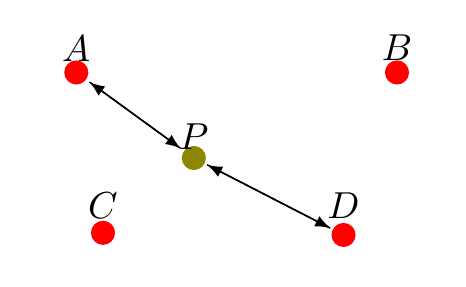
\includegraphics[width=.75\textwidth]{figures/triangle}
 \caption[Closest Directions ] {
 	{\bf Closest Directions}

	}
 \label{fig:triangle}
\end{figure} 

We, then reduce to the three closest directions, so less interpolation weights are to be computed.

One possible way to find the closest three directions is to compute the distance between $P$ and all other four directions and to discard the furthest one.
However, this is computational heavy for real-time applications.
The less computational demanding way is to approximately find the triangle to which $P$ belongs, i.e. $ABC$ or $CBD$.
The following method produces unnoticeable differences of visual results compared to the method which tests if the point $P$ belongs to $ABC$ or $CBD$.


We compute to which direction $P$ is closer, i.e. whether to $A$ or $D$. The distance is computed as follows:

{\centering$d=\sqrt{(x-x^{'})^2+(y-y^{'})^2+(z-z^{'})^2}=
\sqrt{r^2+r^{'2}-2rr'({\color{blue} sin(\theta)sin(\theta^{'})}{\color{magenta}cos(\phi)cos(\phi^{'})}+{\color{blue} sin(\theta)sin(\theta^{'})}{\color{magenta} sin(\phi)sin(\phi^{'})}+cos(\theta)cos(\theta^{'}))}=
\sqrt{r^2+r^{'2}-2rr'({\color{blue} sin(\theta)sin(\theta^{'})}{\color{magenta}cos(\phi-\phi^{'})}+cos(\theta)cos(\theta^{'}))}$\\}


Note that, in practice $r$ and $r^{'}$ are equal 1. As we are interested in comparing distances it is enough to compare this term: 

{\centering$d^{'}=sin(\theta)sin(\theta^{'})cos(\phi-\phi^{'})+cos(\theta)cos(\theta^{'})$\\}

The bigger the term  $d^{'}$ the smaller the overall distance.
If $P$ is closer to $A$, the resulting three directions are $A$, $B$, $C$.
If $P$ closer to $D$ then $B$, $C$, $D$.

If the input direction $P$ is beyond the measuring directions, i.e. $\theta_p>\Delta \theta*n$ for any $n$.
We take the two closer directions, i.e.  $C=(\theta_{U},\phi_{L}^2)$ and $D=(\theta_{U},\phi_{U}^2)$ and perform linear interpolation between these two directions.


\subsection{Barycentric Coordinates}
\label{chapter:barycentric}
A common interpolation technique for the BTF is barycentric coordinates interpolation. 
However, as it is computational heavy, the approximation algorithm proposed by Hatka and Haindl \cite{btfblender} will be used.

Assume that a triangle $P_{1}P_{2}P_{3}$ bounds input point P, for which we want to compute interpolation weights. 
Figure \ref{fig:acquisition_example} demonstrates the hemisphere on which triangle $P_{1}P_{2}P_{3}$ lies.
$C_{P}$ denotes desired pixel color. 
In general, linear interpolation of that pixel will be $C_{P}=w_{1}C_{P1} + w_{2}C_{P2} + w_{1}C_{P2}$, 
where $C_{P1},C_{P2},C_{P3}$ correspond to color values of the found triangle $P_{1}P_{2}P_{3}$ and $w_{1},w_{2},w_{3}$ are normalized and sum up to $1$.

The weights  $w_{1},w_{2},w_{3}$ are defined as volumes $V_{1},V_{2},V_{3}$, which correspond to the tetrahedrons $PP_{2}P_{3}O$, $PP_{3}P_{1}O$, $PP_{1}P_{2}O$, where $O=(0,0,0)$.
These volumes can be calculated as determinants:  

{\centering $w_{1}:=V_{1}=\frac{1}{6}\left | det(PP_{2}P_{3}O) \right |$ \\}
{\centering $w_{2}:=V_{2}=\frac{1}{6}\left | det(PP_{3}P_{1}O) \right |$ \\}
{\centering $w_{3}:=V_{3}=\frac{1}{6}\left | det(PP_{1}P_{2}O) \right |$ \\}

The last step is the normalization, i.e. $V_{i}=\frac{V_{i}}{\sum_{i=1}^{3}V_{i}}$.


\subsection{Algorithm}
\label{chapter:interp_algo}

Computing interpolation weights for the input direction $P$, requires the closest measured directions $P_{1}P_{2}P_{3}$.
After these three directions are known for the input direction $P$, interpolation weights can be computed
as explained in Chapter \ref{chapter:barycentric}.
  
To compute the final interpolated color we combine interpolation weights of light and camera directions.
Assume that $I$ and $O$ are light and camera directions. 
Then, bounding triangles for both of them are $I_{1}I_{2}I_{3}$ and $O_{1}O_{2}O_{3}$ accordingly.
The corresponding barycentric weights are $b_{i}=[b_{i1},b_{i2},b_{i3}]^T$ and $b_{o}=[b_{o1},b_{o2},b_{o3}]^T$.
The final color calculated as the linear combination of $b_{i}$, $b_{o}$ weights and the  measured color values 

 {\centering $ C_{f}=\sum_{u=1}^{3}b_{iu}\sum_{v=1}^{3}b_{ov}C_{uv},$\\} where $C_{uv}$ is a color value that corresponds to a light direction $I_{u}$ and a camera direction $O_{v}$.


\clearpage

\chapter{Implementation}

This chapter describes details, problems and limitations of the thesis implementation part.

The implementation of the demo-application is divided into three main parts: compression, streaming and rendering.
The compression is implemented as a standalone Java application, which compresses BTFs from the Bonn University \cite{btfBonn}.
It is possible to adapt any other BTF databases for our demo-application by resampling BTFs \cite{resampling}.
For streaming we use  Node.js \cite{nodejs} platform.
To integrate 3D graphics into HTML page we use XML3D \cite{xml3d}.
The overall model of the demo application is depicted in Figure \ref{fig:overview}.

\begin{figure}[h]
 \centering
 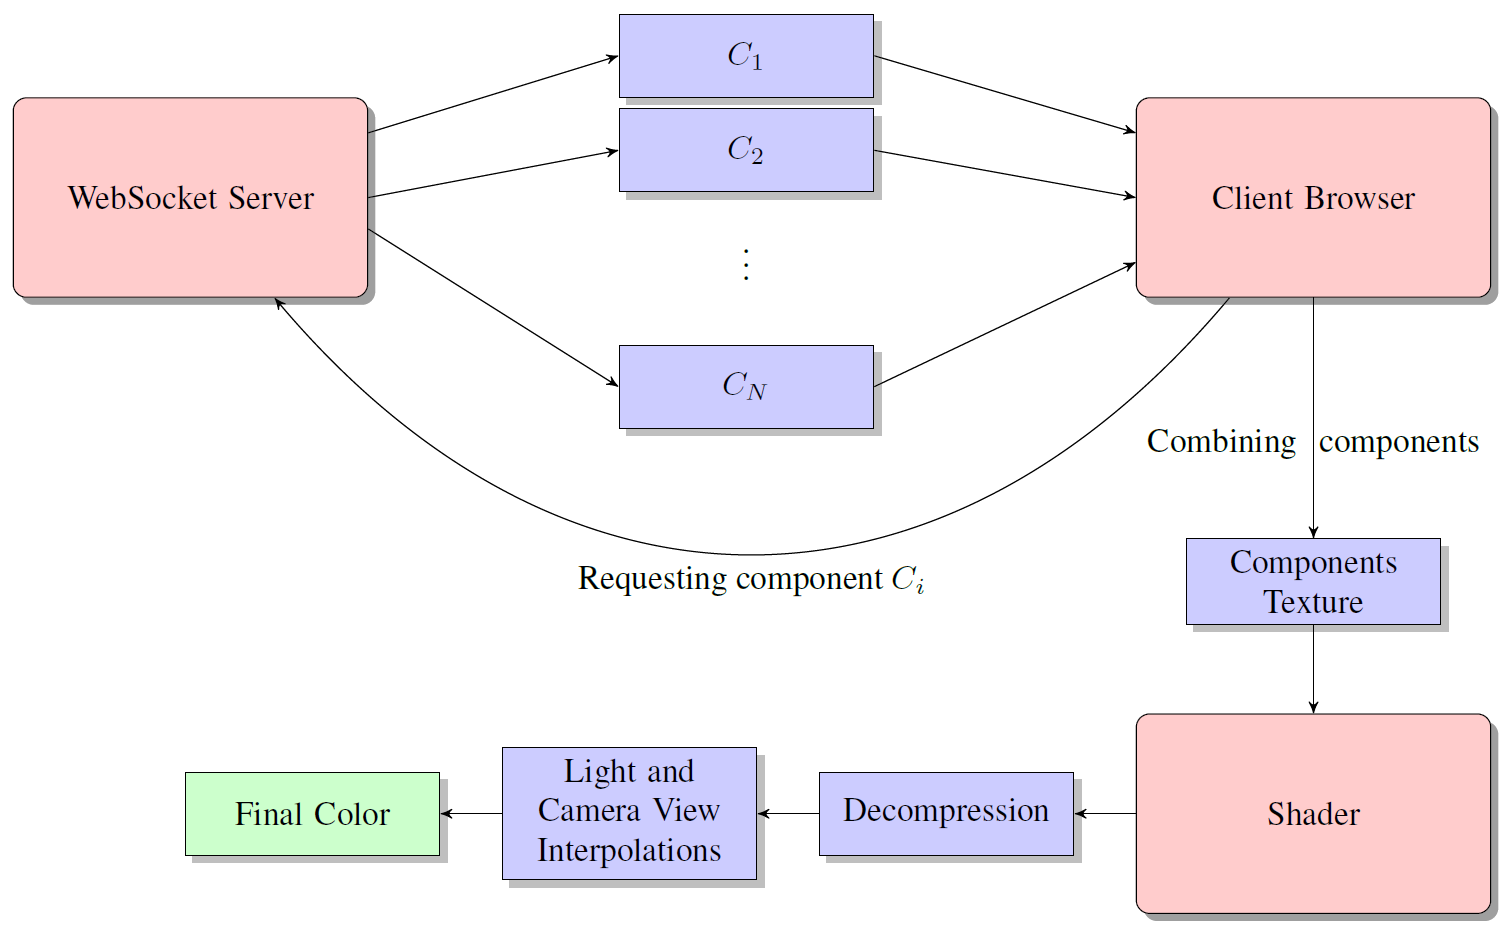
\includegraphics[width=1.0\textwidth]{figures/overview}
 \caption[Model Overview ] {
 	{\bf Model Overview}

	
	}
 \label{fig:overview}
\end{figure}



\section{Compression}
\label{section:impl_compression}

The implementation of the singular value decomposition (SVD) is the main part of the PCA implementation.
 We use \emph{jblas} \cite{jblas} library developed by Mikio Braun. 
 This is a linear algebra library written in Java language, which provides very high performance  \cite{jblas}.
 
The compressed BTFs  have to be sent to the shader. 
  OpenGL Shading Language (GLSL) version 1.0 support uniform arrays, however, they do not fully support dynamic indexing  \cite{glsl}.
Fortunately, it is possible to send arrays of data which are mapped to textures. 
After performing SVD, resulted matrices $U$, $\Sigma$, $V$ are saved as PNG images. (See Chapter \ref{chapter:implementation}).
Values of matrices $U$ and $V$ are in the range of $[-1;1]$.
 Those values have to be mapped to the image domain, i.e. $[0;1]$.
The following function is used to map the values:  

{\centering$f(x)=(x+1)/2$\\}


 Each component of the matrix $U$ is stored as the PNG image.
 For example, if compressed BTF data has $C$ principal components, then this would result in $C$ separate images.
 This is done for streaming purpose, so then principal components can be sent one by one from the server to the client.
 We use  RGBA color space to save four components into the one pixel, because it is possible to do efficient multiplication in the shader by using vector multiplications.
Matrices $V$ and $\Sigma$ are saved in the single shared texture, as they are small in size.

 The matrix $\Sigma$ is a diagonal matrix.
 The values of $\Sigma$ can be bigger than the image color value, i.e. an 8-bit value.
 In practice the values of $\Sigma$ for Bonn University BTFs \cite{btfBonn} are not bigger than four digit number $a_{4}a_{3}a_{2}a_{1}$.
We split the value into two values, i.e. 
 
{\centering$ \underbrace{a_{4}a_{3}}_{R} \underbrace{a_{2}a_{1}}_{G}$\\}
 
It means that two values of $\Sigma$ are mapped into the one pixel, i.e.  one value to RG  channels and the second to BA channels.
If the value of  $\Sigma$ exceed the four digit number, then it is possible to adapt this technique further in the similar manner.


We noticed that in case of Bonn Database \cite{btfBonn} the \emph{jblas} \cite{jblas} library produces relatively sparse values for $U$ and $V$, i.e. close to the zero.
 We scale the data to improve the floating point error caused by mapping of $U$ and $V$ back-and-forth.
The scaling improved the overall decompression error approximately by $5\%$.
 Using the following function we find the scaling factor:
 
 {\centering$ factor(M)=10^{floor(min[log10(min(M)),log10(max(M)]))}$ \\}
 
 where M is the matrix $U$ or $V$. The term $floor(min[log10(min(M)),log10(max(M))])$ calculates the degree with which it is possible to multiply the matrix and preserve the original values range, i.e. $[-1;1]$.
 If it is not possible, the resulting factor will be $1$.
As the decompression is computed as multiplication of $U\Sigma V$, we have to remain the original decompressed BTF values.
We do this by  multiplying each time $\Sigma$ values by the factor $\tfrac{1}{factor(M)}$ if we scale either $U$ or $V$.


 
\section{Streaming}
\label{section:impl_streaming}


We use Node.js \cite{nodejs} as a server side platform, which enables realtime streaming using WebSockets. On top of that, we use BinaryJS \cite{binaryjs} for the binary streaming.
BinaryJS is a framework that uses WebSockets to stream the binary data to the client from the Node.js server.
The server and the client applications are written in JavaScript.



\begin{figure}[h]
 \centering
 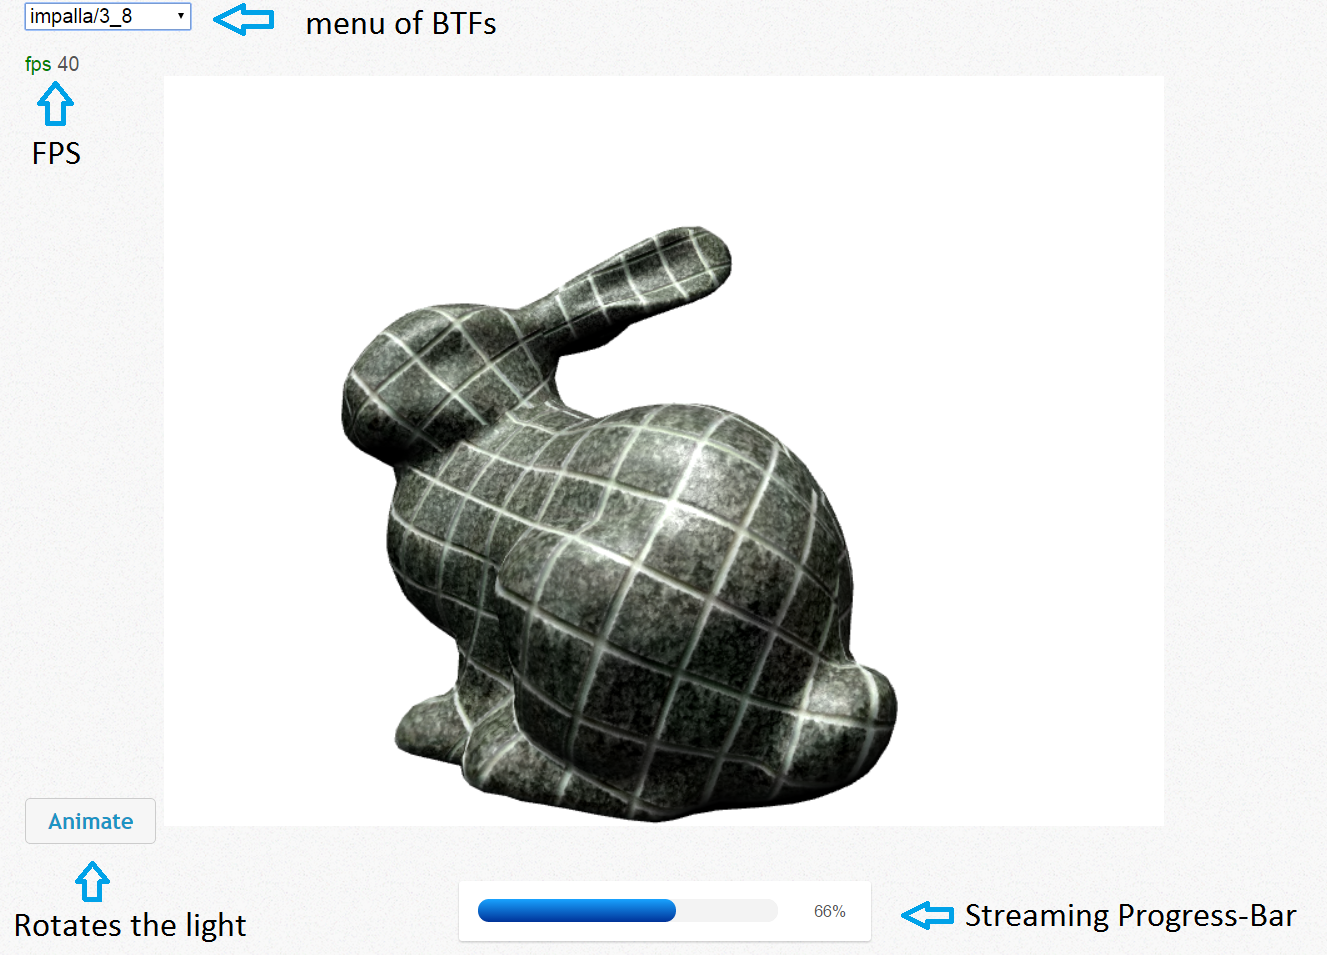
\includegraphics[width=1.0\textwidth]{figures/progress-bar}
 \caption[The streaming progress on the client side] {
 	{\bf The streaming progress on the client side }

 }
 \label{fig:progress-bar}
\end{figure}

We also use Xflow \cite{xflow}, which is a declarative language for data flow processing in realtime.
Xflow is a part of XML3D implementation. We use Xflow for gathering all the transferred principal components and storing them in one common texture $L$. (See Chapter  \ref{section:decompression}).

Consider Figure \ref{fig:streaming} from the Chapter \ref{chapter:streaming} that depicts how the streaming works on practice.
When the user connects to the streaming server and the HTML page loads completely, i.e. all the 3D objects are on the client side, the JavaScript client side sends the message to the Node.js server to start streaming the BTF data.
All the compressed BTFs are located on the Node.js server.
At the start of the stream, we first send texture $R$ and meta data. (See Chapter  \ref{section:decompression}).
Afterwards, each principal component $C_{i}$ are streamed in chunks one by one as PNG images.
Each $C_{i}$ covers all the angular domain, i.e. all the possible camera and light directions.

We decode PNG images using PNG decoder written by Arian Stolwijk \cite{pngreader}. PNG images are decoded to the array of RGB colors and saved to the common texture $L$ in canvas format using Xflow.
Each time the texture $L$ updates the rendering also refreshes.
Even with the first principal component the resulted image looks plausible.
With further components the overall quality of the image improves, i.e. specularities are increasing, small micro-structures become more visible and emphasized.
The user also  able to see the progress-bar of the streaming progress as shown in  Figure \ref{fig:progress-bar}.



Currently the limitation of such streaming approach is the drop of the frame rate when the assembling of the principal components occurs on the client side.
This is caused by the update of the canvas element (texture $L$) each time new component is transmitted to the client.
Also, we did not test the performance of multiple streaming, i.e. if there are several 3D objects that request BTFs at the same time.
 Our current implementation does not support this.
This can be included to the future work. 

\section{Rendering}
\label{section:impl_rendering}


We use XML3D \cite{xml3d} platform to embed 3D graphics into the HTML page. XML3D based on XML and allows for declaring your own 3D scenes and shaders.
XML3D is based on WebGL and JavaScript.

The shader design is depicted in Figure \ref{fig:shader}.
The compressed BTF data comes to the shader in the form of two textures. 
The first texture $L$ stores principal components and the second $R$ stores PCA weights. (See Chapter \ref{section:decompression}).
First, we find three closest directions for the camera and light directions. (See Chapter \ref{chapter:finding_triangle}).
Then, we compute barycentric coordinates for interpolation as described in Chapter \ref{chapter:barycentric}.

\begin{figure}[h]
 \centering
 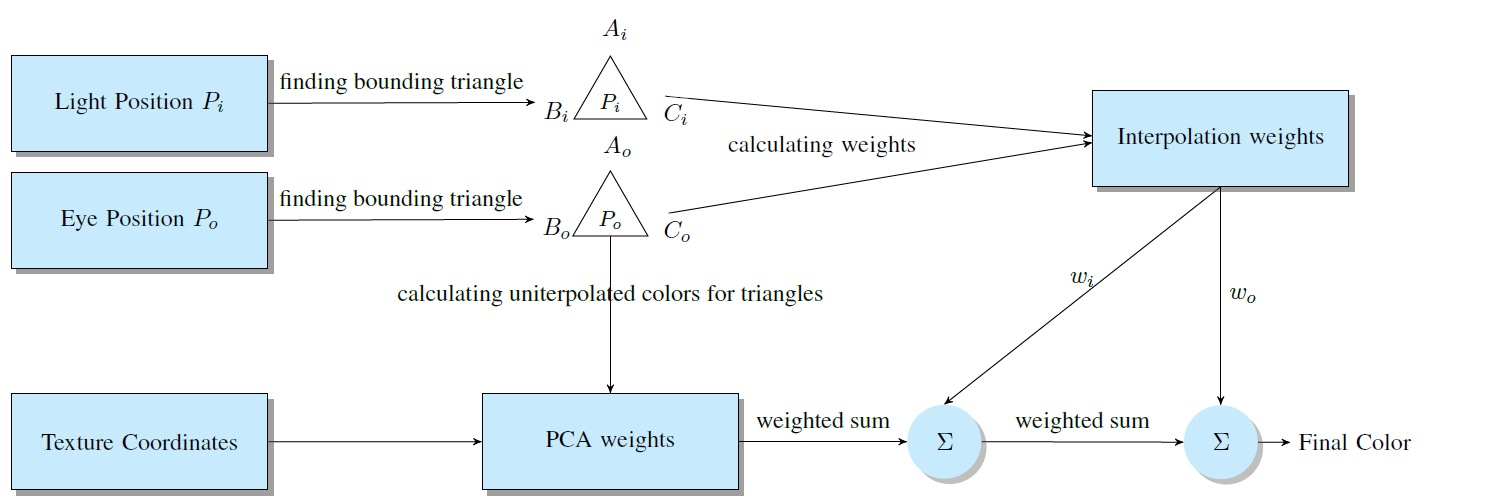
\includegraphics[width=1.0\textwidth]{figures/shader}
 \caption[Shader Design] {
 	{\bf Shader Design }

 }
 \label{fig:shader}
\end{figure}


In the next step we sample the input textures to decompress the needed values for found closest directions.
We have three closest directions per camera and light directions. This means for the interpolation we need to have nine color values. 
For a given texture coordinates $u,v$ we lookup the index of the first principal component, with which it will be possible to start the decompressing.
All the principal components are written linearly in texture $L$, i.e. one by one. 
We have the following mapping to get the needed index:

{\centering$indexL(i,j)= (b*N^2+ (i*N+j))*C$ \\}

where $i=\left \lfloor u*N\right \rfloor$, $j=\left \lfloor v*(N) \right \rfloor$, $b$ is the number of subsets, $N$ is the size of the compressed image and $C$ is number of components.
The parameter $b$ depends on the number of subsets on which PCA is separately done. (See Chapter \ref{section:algorithm_step}).

Texture $R$ stores PCA weights, we lookup the index of suitable compressed image.
The mapping depends on the camera direction $v=(\theta_v,\phi_v)$ and light direction $l=(\theta_l,\phi_l)$.
 It is defined as:

{\centering$ indexR(v,l)=offset(\theta_v,\phi_v)+offset(\theta_l,\phi_l)$\\}

where  $offset(\theta,\phi)=(\tfrac{\theta}{\Delta\theta}+\tfrac{\phi}{\Delta\phi})$, where $\Delta\theta$ and $\Delta\phi$ are quantization step sizes.

When all the indices are computed and textures L and R can be sampled, we decompress the colors as defined in Chapter \ref{section:decompression}.


In a final step we combine nine decompressed colors and early found interpolation weights to get the final color. (See Chapter \ref{chapter:interp_algo}).

The implemented shader has it's own limitations. First of all, the number of principal components has to be fixed for a shader, because GLSL version 1.0 does not allow for dynamic looping \cite{glsl}.
Secondly, the number of principal components are bound by a size of the texture $L$. It means that not all GPUs can handle very big textures. The problem can be fixed by using multiple textures.
But anyway these limitations does not directly influence the performance of the shader, which provides real-time frame rate and performs well even on the mobile devices. (See Figure \ref{fig:progress-bar}).






 




\clearpage

\chapter{Evaluation}
\label{chapter:Evaluation}
In this chapter we will evaluate the presented solution in regard to the decompression error, compression ratio and image quality and real-time performance during the streaming.


\section{Compression}
\label{section:eval_compression}


We evaluate our compression approach using the Bonn's BTF Database \cite{btfBonn} and compare the results to other related PCA methods \cite{haindl}.

We tested different configurations for the BTF compression and decided that the optimal configuration for our method is when $k=3$ and $C=8$, 
where $k$ is the number of neighbour directions and $C$ is the number of principal components. (See Chapter \ref{section:algorithm_step}).
Figure \ref{fig:compression_example} shows an example of the wool material decompressed with various number of components. The Mean Average Error (MAE) in CIELAB color space is computed for each of them.
The CIELAB metrics accounts for the human visual sensitivity, i.e. is consistent with human perception \cite{cielab}.
MAE is calculated for each of the channels separately and then the final result is averaged over them.

{\centering $MAE = \frac{1}{N}\sum_{i=1}^{N}(\left | y_i-\hat{y_i} \right |)$\\}

\begin{figure}[h]
 \centering
 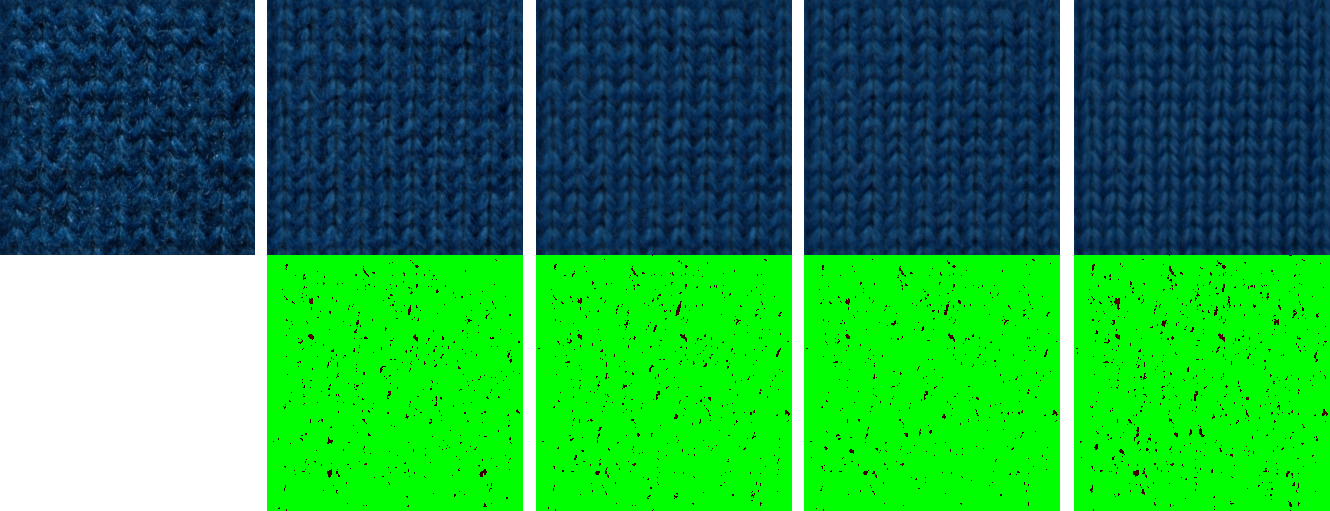
\includegraphics[width=1.0\textwidth]{figures/differ}
 \caption[Example of decompression errors ] {
 	{\bf Example of decompression errors }

	\textbf{First row} from the left to the right: ground truth, \textbf{32} components (MAE:2.17), \textbf{16} components (MAE:1.83), \textbf{8} components (MAE:2.21), \textbf{4} components (MAE:3.04). 
	\textbf{Second row}: the difference between the original and the decompressed images, \emph{red} color denotes how big the error, \emph{green} denotes that the error is absent or very small.}
 \label{fig:compression_example}
\end{figure}




 Figure \ref{fig:compression_example} shows that the decompression error is not significantly improved for $16$ or even $32$ components.
4 Components on the other hand result in a blurred image. This shows that our choice for 8 components is reasonable.
 Haindl \cite{haindl} also claims that $8$ components is the optimal number of components for the PCA RF method, which is related to our method.



 
\begin{table}[h]
\begin{tabular}{|l|l|l|c|c|c|c|c|}
\hline
     & k                      & C                      & \begin{tabular}[c]{@{}c@{}}MAE\\  CIELab\end{tabular} & \begin{tabular}[c]{@{}c@{}}MAE \\ RGB\end{tabular} & \begin{tabular}[c]{@{}c@{}}RMSE\\  RGB\end{tabular} & \multicolumn{1}{l|}{Compression Ratio} & \begin{tabular}[c]{@{}c@{}}Parameters Size /\\  Storage Size (PNGs)\end{tabular} \\ \hline
wool & \multicolumn{1}{c|}{1} & \multicolumn{1}{c|}{8} & 2.14                                                  & 5.86                                               & 7.5                                                 & 1:23                                   & 53Mb / 20 Mb                                                                     \\ \hline
wool & 3                      & \multicolumn{1}{c|}{8} & 2.19                                                  & 6.83                                               & 8.68                                                & 1:70                                   & 18Mb / 5Mb                                                                       \\ \hline
wool & 3                      & 32                     & 2.22                                                  & 5.92                                               & 7.5                                                 & 1:17                                   & 70Mb / 25Mb                                                                      \\ \hline
\end{tabular}
\caption{ Evaluation of BTFs}
\label{table:mytable}
\end{table}


 Table \ref{table:mytable} provides the evaluation for the whole BTF space of the wool sample, i.e. for all possible camera and light directions.
 The MAE is also computed in RGB color space along with the Root Mean Square Error to measure the variance in the errors
 
 {\centering $RMSE = \sqrt{\frac{1}{N}\sum_{i=1}^{N}(y_i-\hat{y_i} )^2}$\\}

 RMSE gives large weights to big errors, thus we can evaluate if big errors are present \cite{rmse}.
 The bigger the RMSE the bigger the variance of the errors. We can see that in our case the RMSE is close to the MAE, which means that the variance of the errors is relatively small.
 
In the first row of the  Table \ref{table:mytable} where $k=1$ our method becomes equal to the PCA RF \cite{haindl} method.
Haindl \cite{haindl} claims to have the MAE equal to $3.16$ in CIELAB color space for the same sample.
 Our method produces better result, i.e. $2.14$. 
 The second row shows that for  $k=3$ MAE stays practically the same. 
 However, the compression ratio improves by a factor of three.
 We can see that even for $32$ components the decompression errors improves only insignificantly, but the compression ratio becomes worse.
 If we use $k>3$, more components would be necessary to reduce decompression errors.
 For intance, our method becomes equal to the PCA BTF \cite{haindl} method if $k=81$ (all camera directions). 
 In this case approximately $41$ components are necessary \cite{haindl}.
 
 Also, the LPCA BTF \cite{haindl} method uses $19$ components on average and has the MAE equal to $2.42$, while our method uses $8$ components.
 
 

\section{Real-time performance}
\label{section:eval_streaming}


We evaluate the rendering quality during the streaming and the real-time performance.
Figure \ref{fig:streamPreview} depicts intermediate images during the streaming.
We tested our approach on three materials: wool, impalla and corduroy.
The parameters for the compression are $k=3$ and $C=8$.

\begin{figure}[h]
 \centering
 \includegraphics[width=.87\textwidth]{figures/streampreview}
 \caption[Example of Progressive Streaming ] {
 	{\bf Example of Progressive Streaming}

	\textbf{From left to right}: \emph{1}, \emph{2}, \emph{4}, \emph{6}, \emph{8}  components rendered accordingly.
	}
 \label{fig:streamPreview}
\end{figure}
\label{chapter:implementation}



\begin{figure}[h]
 \centering
 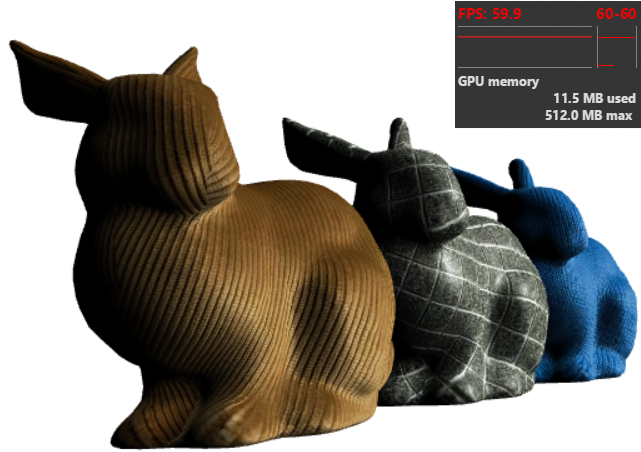
\includegraphics[width=.65\textwidth]{figures/3BTFs}
 \caption[Example of 3 BTFs rendered at the same time ] {
 	{\bf Example of 3 BTFs rendered at the same time }

	\textbf{From left to right}: corduroy, impalla and wool materials are rendered under dynamic light.
	}
 \label{fig:3BTFs}
\end{figure}
\label{chapter:implementation}

Rendering starts as soon as the first component transfers to the client side.
 The overall appearance of the the material is already visible even with the first the component, which has an average size of about $0.7$Mb.
With further components the overall quality of the image improves, i.e. specularities are increasing, small micro-structures become more visible and emphasized.
On a desktop computer with a NVIDIA GeForce GTX 480 graphics card 3 BTFs can be rendered at 60 frames per second.
Figure \ref{fig:3BTFs} shows an example of this.

On a Sony Xperia SL 15 frames per second are achieved on average for one BTF at a time.


\section{Comparison with the Phong Shader}
\label{section:eval_streaming}

Figure \ref{fig:phongvsbtf} shows the tremendous difference between the BTF and a conventional 2-D texture in combination with the Phong shader.
Both images were taken under the same camera and light directions. The BTF introduces high varying specularities and the realistic depth in the images.
The Phong shader with the combination of the 2-D texture provides the impression that the material looks flat.
The BTF shows the correct inner-reflections, sub-surface scattering and shadows under varying light conditions.

\begin{figure}[hb]
 \centering
 \includegraphics[width=.73\textwidth]{figures/phongVsBTF}
 \caption[The Phong model in comparison to the BTF ] {
 	{\bf The Phong model in comparison to the BTF  }
	}
 \label{fig:phongvsbtf}
\end{figure}


\clearpage

\chapter{Conclusions and Future Work}
\label{chapter:conclusions}
 Bidirectional Texture Functions are currently the best texture representation for the materials 
 that contain high frequencies both in the angular and spatial domain \cite{mueller-2003-compression}.
 Thousands of images has to be taken to sample the appearance of such materials.
 Due to huge sizes of acquired BTFs real-time rendering is impossible to achieve without suitable compression.
 Thus, BTFs still staying in a state of the art in computer graphics. 

\section{Summary}

 In this work we achieved real-time rendering of BTFs in a high quality.
 Considering that we render BTFs in a browser, we managed to reduce the latency that is caused by the data transmission, i.e.
 by streaming  principal components individually.
 We are able to show immediately intermediate rendering results of the textured 3D object.
 We showed experimentally that it is possible to improve the decompression error that was caused by floating point imprecisions.
 The scaling of the compressed BTF data before converting it into the textures improved the decompression error approximately by $5\%$.
 As a result this also improved the real-time frame rates and the compression ratio due to reduction in the number of components used.


Finally, our method is flexible and allows for balancing between the visual quality, memory usage and computational effort.
\section{Future work}
\label{section:future_work}

Based on our results several directions for the future work can be made.
First of all, multiple streaming of BTFs can be implemented.
Secondly, several optimizations of the BTF shader performance can be made.
For instance, it is possible to reduce some of the calculations such as computation of the interpolation weights. 
They can be precomputed and stored in a cube-map \cite{haindl}.
Other calculations such as computation of the bidirectional normals can be precomputed and stored along with a 3D mesh.

Last but not least, there is a room for further compression.
 For instance, it can be achieved by compressing the PCA parameters with wavelet compression \cite{webglbtfstreaming} or with entropy encoding \cite{gpu_gems}. 
However, the decompression cost will grow, but it can be worth if further memory savings are necessary. 
\clearpage


% *************** Bibliography ***************
\bibliographystyle{plain}
{\small\bibliography{references}}
\clearpage



% *************** Back matter ***************
%\backmatter
%\input{back.tex}

\end{document}